\chapter{Implementation in Julia}\label{ch:julia}

% framework
I first implemented a set covering machine with single threshold base classifiers, such as rays, in order to extend it in the following chapters.
This was done in Julia, a fast and simple structured programming language first presented in~\cite{bezanson}, in version 1.7.2.
Furthermore the packages `\texttt{CVS.jl}' and `\texttt{RData.jl}' to read CSV and RData files, in addition to
`\texttt{DataFrames.jl}' for the efficient and comfortable handling of data matrices, were employed.
In contrast to a usual Julia matrix, each column of a data frame has a distinct name, that can be set by the user.
`\texttt{PlotlyJS.jl}' was used as the graphing library for plotting the results and
`\texttt{BenchmarkTools.jl}' for benchmarking with the `\texttt{@btime}' macro to log execution times and used RAM spaces.

% good performance
After starting with the BuildSCM algorithm of~\cite{marchand02} with binary features as the fundament,
the basis algorithm is then adjusted and optimized for the computation in Julia, in order to improve its run time performance,
i.e.\ to minimize the algorithm's execution time and its RAM workload.
This is needed as, in the end, the SCM shall be capable of analyzing huge data sets with up to 50,000 features and a few hundred samples.

\section{Adjusting the BuildSCM Algorithm}

\begin{figure}[ht]
    \centering
    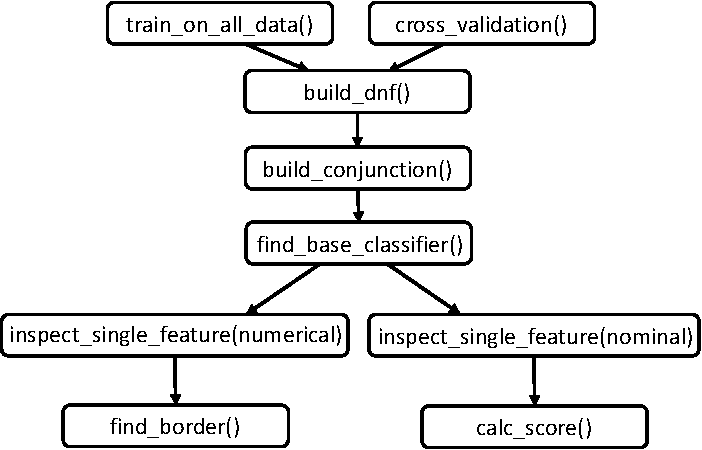
\includegraphics[width=0.85\columnwidth]{figures/training_structure.pdf}
    \caption{Structure of the training algorithm. \autoref{ch:dnf} will explain the need and details of the \texttt{build\_dnf} function. While \autoref{ch:varFeat} will explain the reasons for splitting the \texttt{inspect\_single\_feature} function.}\label{fig:training_structure}
\end{figure}

\begin{jllisting}[caption={Storing base classifiers as structs.}, label={julia:baseClassifier}]
    struct BaseClassifier
        featureId::Int32
        operator::Char
        threshold::Union{Float64, Int64, Bool, AbstractString}
        score::Float64
    end
\end{jllisting}

I structured my SCM training algorithm as displayed in \autoref{fig:training_structure}.
In contrast to the usage of a binary direction variable for rays like in the original algorithm of~\cite{marchand02}, a Julia struct `BaseClassifier' (see \autoref{julia:baseClassifier})
is now used to store each ray's attributes in a central, immutable and easy to understand structure.
As the rays's operator is stored as an arbitrary char, a function to interpret it, in the style of `\texttt{if operator == '\(\geq\)' then return value < threshold}', is needed additionally.
Yet, besides this and a slightly increased RAM and execution time demands, this form of storage comes with the huge advantage of being extendible to many different kinds 
of rays and even other base classifiers, for example for the integration of an `=' or an `>' operator, as done in \autoref{ch:varFeat}.

% low level to high level
For the calculation of each base classfier's usefulness score, implemented in \autoref{julia:calcScore}, 
the formula suggested by~\cite{marchand02} with a constant value for \(p\) is used and
no further investigations on other functions to calculate this score are performed.
However \(Q\) and \(R\) are computed adhoc, without the use of any \(N\) or \(P\), as done by~\cite{marchand02}.
In general, it is quite insufficient to handle \(Q\) and \(R\) as the real rows of the data matrix \(S\), as with this
method execution times skyrocket, already when dealing with slightly larger data sets.
The next option would be to handle \(Q\) and \(R\) in the form of indices that reference the corresponding lines of \(S\).
However this approach is also not feasible in the context of big data sets, as the constant storing,
transferring and updating of these parameters leads to way too much computational effort.
Instead it is best to simply recalculate the usefulness score together with \(Q\) and \(R\) whenever it is needed.
This decreases the code's RAM requirements from \(\mathcal{O}(|\text{features}| \cdot |\text{samples}| \cdot 2)\) for permanently storing the current Q and R indices
of all features for possibly all samples, to only \(\mathcal{O}(1)\) for storing the element with the maximum score at the time.

The best base classifiers are then collected and compared to each other on different tiers of the algorithm.
Finally, in each iteration the optimal classifier is chosen and incorporated into a classifier that works purely conjunctive.
The next iteration of the \texttt{build\_conjunction} function, depicted in \autoref{julia:buildConj},
then continues on the samples that were classified as positive by all previously selected base classifiers, as well as the new ones.
However, once a base classifier, that does not classify at least one positive and one negative
sample correctly, is selected as the new optimum, this classifier is discarded and the conjunction is finished right away.
This ensures that the conjunction will not grow without a good reason to do so.

\section{Performance Optimization}

% pretty code and efficient
In general great emphasis was put on creating compact, maintainable and well documented Julia code.
However, at the same time, the SCM was also designed to be as high performant as possible,
in order to be able to test it on huge data sets later on.
To achieve these goals, many performance optimized Julia features were used, such as multiple dispatch, Julia's version of function overloading,
anonymous parameters `\_' and a strong typing system that is used for all function parameters.

While using fixed-length tuples instead of vectors seemed promising at first, it did in fact not turn out
too well, as the data set is loaded from its original file as a data frame either way.
From this data frame, single vectors are easily extractable, but to obtain tuples, the corresponding vectors have to be
re-typed manually --- a process, which is quite performance intense.
Therefore mainly data frames and vectors were used in the end, yet there are still multiple ways to optimize them, like
referencing a column by using `\texttt{S[!, x]}' instead of copying it by `\texttt{S[:, x]}' and only passing essential
data to subfunction, like pre-extracted vectors or values.
Sets, instead of arrays, were employed wherever they were useful, in order to be able to use efficient Julia operations especially designed for sets, such as `\texttt{union}' and `\texttt{setdiff}'.
Those operations are in general faster than the the equivalent operations on arrays. 

% interpretable rules
Moreover I put effort in producing easy to interpret classification rules.
Instead of outputting confusing tables, like some other SCM algorithms do, my algorithm actually outputs
the whole rule in a human readable form like `\texttt{IF length < 5.1 AND height < 7.3 THEN will fit}'.
In these rules real feature names, instead of their their abbreviations, and real class names, instead of just `class 1' and `class 0',
were used.
This ensures that the SCM is able to produce rules that can eventually be supported or validated by science, as suggested~\cite{drouin16}.

However to keep the algorithm at high performant as possible, the calculations were done on the feature's indexes and Boolean class labels themselves and
the semantic details were solely solely when needed.
In case of the feature names, that task is done by the \texttt{to\_string} functions, as displayed in \autoref{julia:toString}.
This group of functions is also a prime example for the use of multiple dispatch.
For the class labels, on the other hand, the Julia function \texttt{booleanize\_labels!} (see \autoref{julia:boolLabels}) was used to extract the labels
from the loaded data and obtain a data frame with Boolean labels.
This data frame is then suitable for an ensemble of highly efficient vector operations and compact enough for quick transferring to various functions.

% Parallelization by multi threading
Furthermore parallelization was incorporated by starting Julia with the command `\texttt{julia --threads auto}'
and using the `\texttt{Threads.@threads for i in 1:m}'\\macro to activate multi threading in certain loops.
Within a multithreaded loop, it is important to ensure the independence of each iteration, i.e.\ if
a variable is manipulated by a thread, it may not be manipulated, or even read, by any other thread.
Therefore fixed width arrays were used, where every thread has its own array position that it can write to.

Within the SCM, parallelization was especially useful at the \(m \times n\) iterations of a cross-validation (see \autoref{sec:evalMethods})
and within the \texttt{find\_base\_classifier} function,
as in these use cases, every iteration constructs a model that is completely independent from all other iterations.
\texttt{Find\_base\_classifier} in particular collects the optimal base classifier of every feature, compares them and returns only the best, i.e.\ the highest scoring, of them.
Its multithreaded implementation can be found in \autoref{julia:findBaseClassifier}.
The parallelization drastically improves the algorithms runtime performance:
When executing the \texttt{build\_conjunction} routine with a randomly generated data set of 50,000 numerical features and 200 samples,
it needs about 22.734 seconds without and 8.855 seconds with multithreading used in the \texttt{find\_base\_classifier} function.